\documentclass[1p]{elsarticle_modified}
%\bibliographystyle{elsarticle-num}

%\usepackage[colorlinks]{hyperref}
%\usepackage{abbrmath_seonhwa} %\Abb, \Ascr, \Acal ,\Abf, \Afrak
\usepackage{amsfonts}
\usepackage{amssymb}
\usepackage{amsmath}
\usepackage{amsthm}
\usepackage{scalefnt}
\usepackage{amsbsy}
\usepackage{kotex}
\usepackage{caption}
\usepackage{subfig}
\usepackage{color}
\usepackage{graphicx}
\usepackage{xcolor} %% white, black, red, green, blue, cyan, magenta, yellow
\usepackage{float}
\usepackage{setspace}
\usepackage{hyperref}

\usepackage{tikz}
\usetikzlibrary{arrows}

\usepackage{multirow}
\usepackage{array} % fixed length table
\usepackage{hhline}

%%%%%%%%%%%%%%%%%%%%%
\makeatletter
\renewcommand*\env@matrix[1][\arraystretch]{%
	\edef\arraystretch{#1}%
	\hskip -\arraycolsep
	\let\@ifnextchar\new@ifnextchar
	\array{*\c@MaxMatrixCols c}}
\makeatother %https://tex.stackexchange.com/questions/14071/how-can-i-increase-the-line-spacing-in-a-matrix
%%%%%%%%%%%%%%%

\usepackage[normalem]{ulem}

\newcommand{\msout}[1]{\ifmmode\text{\sout{\ensuremath{#1}}}\else\sout{#1}\fi}
%SOURCE: \msout is \stkout macro in https://tex.stackexchange.com/questions/20609/strikeout-in-math-mode

\newcommand{\cancel}[1]{
	\ifmmode
	{\color{red}\msout{#1}}
	\else
	{\color{red}\sout{#1}}
	\fi
}

\newcommand{\add}[1]{
	{\color{blue}\uwave{#1}}
}

\newcommand{\replace}[2]{
	\ifmmode
	{\color{red}\msout{#1}}{\color{blue}\uwave{#2}}
	\else
	{\color{red}\sout{#1}}{\color{blue}\uwave{#2}}
	\fi
}

\newcommand{\Sol}{\mathcal{S}} %segment
\newcommand{\D}{D} %diagram
\newcommand{\A}{\mathcal{A}} %arc


%%%%%%%%%%%%%%%%%%%%%%%%%%%%%5 test

\def\sl{\operatorname{\textup{SL}}(2,\Cbb)}
\def\psl{\operatorname{\textup{PSL}}(2,\Cbb)}
\def\quan{\mkern 1mu \triangleright \mkern 1mu}

\theoremstyle{definition}
\newtheorem{thm}{Theorem}[section]
\newtheorem{prop}[thm]{Proposition}
\newtheorem{lem}[thm]{Lemma}
\newtheorem{ques}[thm]{Question}
\newtheorem{cor}[thm]{Corollary}
\newtheorem{defn}[thm]{Definition}
\newtheorem{exam}[thm]{Example}
\newtheorem{rmk}[thm]{Remark}
\newtheorem{alg}[thm]{Algorithm}

\newcommand{\I}{\sqrt{-1}}
\begin{document}

%\begin{frontmatter}
%
%\title{Boundary parabolic representations of knots up to 8 crossings}
%
%%% Group authors per affiliation:
%\author{Yunhi Cho} 
%\address{Department of Mathematics, University of Seoul, Seoul, Korea}
%\ead{yhcho@uos.ac.kr}
%
%
%\author{Seonhwa Kim} %\fnref{s_kim}}
%\address{Center for Geometry and Physics, Institute for Basic Science, Pohang, 37673, Korea}
%\ead{ryeona17@ibs.re.kr}
%
%\author{Hyuk Kim}
%\address{Department of Mathematical Sciences, Seoul National University, Seoul 08826, Korea}
%\ead{hyukkim@snu.ac.kr}
%
%\author{Seokbeom Yoon}
%\address{Department of Mathematical Sciences, Seoul National University, Seoul, 08826,  Korea}
%\ead{sbyoon15@snu.ac.kr}
%
%\begin{abstract}
%We find all boundary parabolic representation of knots up to 8 crossings.
%
%\end{abstract}
%\begin{keyword}
%    \MSC[2010] 57M25 
%\end{keyword}
%
%\end{frontmatter}

%\linenumbers
%\tableofcontents
%
\newcommand\colored[1]{\textcolor{white}{\rule[-0.35ex]{0.8em}{1.4ex}}\kern-0.8em\color{red} #1}%
%\newcommand\colored[1]{\textcolor{white}{ #1}\kern-2.17ex	\textcolor{white}{ #1}\kern-1.81ex	\textcolor{white}{ #1}\kern-2.15ex\color{red}#1	}

{\Large $\underline{12a_{0476}~(K12a_{0476})}$}

\setlength{\tabcolsep}{10pt}
\renewcommand{\arraystretch}{1.6}
\vspace{1cm}\begin{tabular}{m{100pt}>{\centering\arraybackslash}m{274pt}}
\multirow{5}{120pt}{
	\centering
	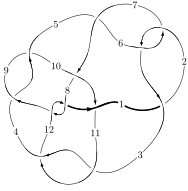
\includegraphics[width=112pt]{../../../GIT/diagram.site/Diagrams/png/1277_12a_0476.png}\\
\ \ \ A knot diagram\footnotemark}&
\allowdisplaybreaks
\textbf{Linearized knot diagam} \\
\cline{2-2}
 &
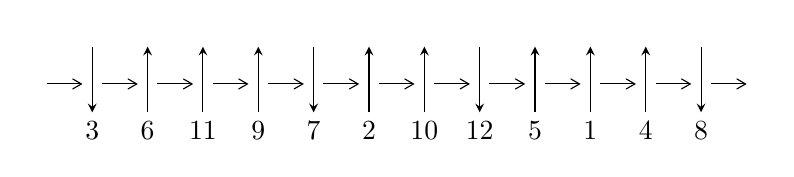
\begin{tikzpicture}[x=20pt, y=17pt]
	% nodes
	\node (C0) at (0, 0) {};
	\node (C1) at (1, 0) {};
	\node (C1U) at (1, +1) {};
	\node (C1D) at (1, -1) {3};

	\node (C2) at (2, 0) {};
	\node (C2U) at (2, +1) {};
	\node (C2D) at (2, -1) {6};

	\node (C3) at (3, 0) {};
	\node (C3U) at (3, +1) {};
	\node (C3D) at (3, -1) {11};

	\node (C4) at (4, 0) {};
	\node (C4U) at (4, +1) {};
	\node (C4D) at (4, -1) {9};

	\node (C5) at (5, 0) {};
	\node (C5U) at (5, +1) {};
	\node (C5D) at (5, -1) {7};

	\node (C6) at (6, 0) {};
	\node (C6U) at (6, +1) {};
	\node (C6D) at (6, -1) {2};

	\node (C7) at (7, 0) {};
	\node (C7U) at (7, +1) {};
	\node (C7D) at (7, -1) {10};

	\node (C8) at (8, 0) {};
	\node (C8U) at (8, +1) {};
	\node (C8D) at (8, -1) {12};

	\node (C9) at (9, 0) {};
	\node (C9U) at (9, +1) {};
	\node (C9D) at (9, -1) {5};

	\node (C10) at (10, 0) {};
	\node (C10U) at (10, +1) {};
	\node (C10D) at (10, -1) {1};

	\node (C11) at (11, 0) {};
	\node (C11U) at (11, +1) {};
	\node (C11D) at (11, -1) {4};

	\node (C12) at (12, 0) {};
	\node (C12U) at (12, +1) {};
	\node (C12D) at (12, -1) {8};
	\node (C13) at (13, 0) {};

	% arrows
	\draw[->,>={angle 60}]
	(C0) edge (C1) (C1) edge (C2) (C2) edge (C3) (C3) edge (C4) (C4) edge (C5) (C5) edge (C6) (C6) edge (C7) (C7) edge (C8) (C8) edge (C9) (C9) edge (C10) (C10) edge (C11) (C11) edge (C12) (C12) edge (C13) ;	\draw[->,>=stealth]
	(C1U) edge (C1D) (C2D) edge (C2U) (C3D) edge (C3U) (C4D) edge (C4U) (C5U) edge (C5D) (C6D) edge (C6U) (C7D) edge (C7U) (C8U) edge (C8D) (C9D) edge (C9U) (C10D) edge (C10U) (C11D) edge (C11U) (C12U) edge (C12D) ;
	\end{tikzpicture} \\
\hhline{~~} \\& 
\textbf{Solving Sequence} \\ \cline{2-2} 
 &
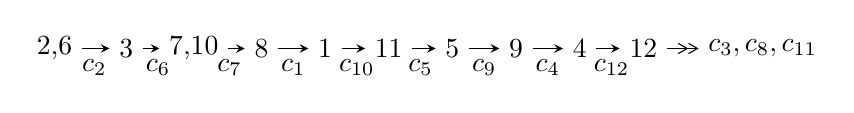
\begin{tikzpicture}[x=23pt, y=7pt]
	% node
	\node (A0) at (-1/8, 0) {2,6};
	\node (A1) at (1, 0) {3};
	\node (A2) at (33/16, 0) {7,10};
	\node (A3) at (25/8, 0) {8};
	\node (A4) at (33/8, 0) {1};
	\node (A5) at (41/8, 0) {11};
	\node (A6) at (49/8, 0) {5};
	\node (A7) at (57/8, 0) {9};
	\node (A8) at (65/8, 0) {4};
	\node (A9) at (73/8, 0) {12};
	\node (C1) at (1/2, -1) {$c_{2}$};
	\node (C2) at (3/2, -1) {$c_{6}$};
	\node (C3) at (21/8, -1) {$c_{7}$};
	\node (C4) at (29/8, -1) {$c_{1}$};
	\node (C5) at (37/8, -1) {$c_{10}$};
	\node (C6) at (45/8, -1) {$c_{5}$};
	\node (C7) at (53/8, -1) {$c_{9}$};
	\node (C8) at (61/8, -1) {$c_{4}$};
	\node (C9) at (69/8, -1) {$c_{12}$};
	\node (A10) at (11, 0) {$c_{3},c_{8},c_{11}$};

	% edge
	\draw[->,>=stealth]	
	(A0) edge (A1) (A1) edge (A2) (A2) edge (A3) (A3) edge (A4) (A4) edge (A5) (A5) edge (A6) (A6) edge (A7) (A7) edge (A8) (A8) edge (A9) ;
	\draw[->>,>={angle 60}]	
	(A9) edge (A10);
\end{tikzpicture} \\ 

\end{tabular} \\

\footnotetext{
The image of knot diagram is generated by the software ``\textbf{Draw programme}" developed by Andrew Bartholomew(\url{http://www.layer8.co.uk/maths/draw/index.htm\#Running-draw}), where we modified some parts for our purpose(\url{https://github.com/CATsTAILs/LinksPainter}).
}\phantom \\ \newline 
\centering \textbf{Ideals for irreducible components\footnotemark of $X_{\text{par}}$} 
 
\begin{align*}
I^u_{1}&=\langle 
-443 u^{40}-3423 u^{39}+\cdots+4 b+532,\;-955 u^{40}-7773 u^{39}+\cdots+8 a+3572,\\
\phantom{I^u_{1}}&\phantom{= \langle  }u^{41}+9 u^{40}+\cdots-12 u-8\rangle \\
I^u_{2}&=\langle 
1.43701\times10^{23} a^{5} u^{10}-4.78586\times10^{23} a^{4} u^{10}+\cdots+3.13902\times10^{22} a+7.88174\times10^{22},\\
\phantom{I^u_{2}}&\phantom{= \langle  }- u^{10} a^5+3 u^{10} a^4+\cdots+13 a+49,\;u^{11}- u^{10}+2 u^9- u^8+4 u^7-2 u^6+4 u^5- u^4+3 u^3+u^2+1\rangle \\
I^u_{3}&=\langle 
u^{26}+3 u^{24}+\cdots+b+3,\;- u^{26}+4 u^{25}+\cdots+a+5,\;u^{27}-2 u^{26}+\cdots-2 u+1\rangle \\
\\
\end{align*}
\raggedright * 3 irreducible components of $\dim_{\mathbb{C}}=0$, with total 134 representations.\\
\footnotetext{All coefficients of polynomials are rational numbers. But the coefficients are sometimes approximated in decimal forms when there is not enough margin.}
\newpage
\renewcommand{\arraystretch}{1}
\centering \section*{I. $I^u_{1}= \langle -443 u^{40}-3423 u^{39}+\cdots+4 b+532,\;-955 u^{40}-7773 u^{39}+\cdots+8 a+3572,\;u^{41}+9 u^{40}+\cdots-12 u-8 \rangle$}
\flushleft \textbf{(i) Arc colorings}\\
\begin{tabular}{m{7pt} m{180pt} m{7pt} m{180pt} }
\flushright $a_{2}=$&$\begin{pmatrix}1\\0\end{pmatrix}$ \\
\flushright $a_{6}=$&$\begin{pmatrix}0\\u\end{pmatrix}$ \\
\flushright $a_{3}=$&$\begin{pmatrix}1\\- u^2\end{pmatrix}$ \\
\flushright $a_{7}=$&$\begin{pmatrix}u\\u\end{pmatrix}$ \\
\flushright $a_{10}=$&$\begin{pmatrix}119.375 u^{40}+971.625 u^{39}+\cdots-884.750 u-446.500\\\frac{443}{4} u^{40}+\frac{3423}{4} u^{39}+\cdots-708 u-133\end{pmatrix}$ \\
\flushright $a_{8}=$&$\begin{pmatrix}-\frac{327}{8} u^{40}-\frac{2569}{8} u^{39}+\cdots+\frac{1063}{4} u+107\\-\frac{121}{4} u^{40}-\frac{863}{4} u^{39}+\cdots+\frac{301}{2} u-47\end{pmatrix}$ \\
\flushright $a_{1}=$&$\begin{pmatrix}u^2+1\\- u^4\end{pmatrix}$ \\
\flushright $a_{11}=$&$\begin{pmatrix}40.1250 u^{40}+295.375 u^{39}+\cdots-200.750 u+4.50000\\\frac{79}{4} u^{40}+\frac{479}{4} u^{39}+\cdots-44 u+91\end{pmatrix}$ \\
\flushright $a_{5}=$&$\begin{pmatrix}u^3\\u^3+u\end{pmatrix}$ \\
\flushright $a_{9}=$&$\begin{pmatrix}-3.62500 u^{40}-21.3750 u^{39}+\cdots-28.7500 u+17.5000\\\frac{31}{4} u^{40}+\frac{403}{4} u^{39}+\cdots-158 u-163\end{pmatrix}$ \\
\flushright $a_{4}=$&$\begin{pmatrix}\frac{9}{8} u^{40}-\frac{57}{8} u^{39}+\cdots+\frac{119}{4} u+92\\-\frac{75}{4} u^{40}-\frac{669}{4} u^{39}+\cdots+\frac{343}{2} u+159\end{pmatrix}$ \\
\flushright $a_{12}=$&$\begin{pmatrix}-\frac{473}{8} u^{40}-\frac{3849}{8} u^{39}+\cdots+\frac{915}{2} u+210\\-46 u^{40}-\frac{689}{2} u^{39}+\cdots+\frac{575}{2} u-33\end{pmatrix}$\\&\end{tabular}
\flushleft \textbf{(ii) Obstruction class $= -1$}\\~\\
\flushleft \textbf{(iii) Cusp Shapes $= 83 u^{40}+505 u^{39}+\cdots-222 u+694$}\\~\\
\newpage\renewcommand{\arraystretch}{1}
\flushleft \textbf{(iv) u-Polynomials at the component}\newline \\
\begin{tabular}{m{50pt}|m{274pt}}
Crossings & \hspace{64pt}u-Polynomials at each crossing \\
\hline $$\begin{aligned}c_{1},c_{5}\end{aligned}$$&$\begin{aligned}
&u^{41}+13 u^{40}+\cdots-432 u-64
\end{aligned}$\\
\hline $$\begin{aligned}c_{2},c_{6}\end{aligned}$$&$\begin{aligned}
&u^{41}-9 u^{40}+\cdots-12 u+8
\end{aligned}$\\
\hline $$\begin{aligned}c_{3},c_{4},c_{9}\\c_{11}\end{aligned}$$&$\begin{aligned}
&u^{41}- u^{40}+\cdots+3 u-1
\end{aligned}$\\
\hline $$\begin{aligned}c_{7},c_{10}\end{aligned}$$&$\begin{aligned}
&u^{41}+3 u^{40}+\cdots+19 u-1
\end{aligned}$\\
\hline $$\begin{aligned}c_{8},c_{12}\end{aligned}$$&$\begin{aligned}
&u^{41}+25 u^{40}+\cdots+33792 u+2048
\end{aligned}$\\
\hline
\end{tabular}\\~\\
\newpage\renewcommand{\arraystretch}{1}
\flushleft \textbf{(v) Riley Polynomials at the component}\newline \\
\begin{tabular}{m{50pt}|m{274pt}}
Crossings & \hspace{64pt}Riley Polynomials at each crossing \\
\hline $$\begin{aligned}c_{1},c_{5}\end{aligned}$$&$\begin{aligned}
&y^{41}+33 y^{40}+\cdots-307968 y-4096
\end{aligned}$\\
\hline $$\begin{aligned}c_{2},c_{6}\end{aligned}$$&$\begin{aligned}
&y^{41}+13 y^{40}+\cdots-432 y-64
\end{aligned}$\\
\hline $$\begin{aligned}c_{3},c_{4},c_{9}\\c_{11}\end{aligned}$$&$\begin{aligned}
&y^{41}-41 y^{40}+\cdots+5 y-1
\end{aligned}$\\
\hline $$\begin{aligned}c_{7},c_{10}\end{aligned}$$&$\begin{aligned}
&y^{41}-25 y^{40}+\cdots+113 y-1
\end{aligned}$\\
\hline $$\begin{aligned}c_{8},c_{12}\end{aligned}$$&$\begin{aligned}
&y^{41}+21 y^{40}+\cdots-7340032 y-4194304
\end{aligned}$\\
\hline
\end{tabular}\\~\\
\newpage\flushleft \textbf{(vi) Complex Volumes and Cusp Shapes}
$$\begin{array}{c|c|c}  
\text{Solutions to }I^u_{1}& \I (\text{vol} + \sqrt{-1}CS) & \text{Cusp shape}\\
 \hline 
\begin{aligned}
u &= \phantom{-}0.606113 + 0.756260 I \\
a &= -0.527663 - 0.015390 I \\
b &= \phantom{-}0.186140 + 0.888970 I\end{aligned}
 & \phantom{-}0.717698 - 0.435826 I & \phantom{-}11.97986 + 0.51850 I \\ \hline\begin{aligned}
u &= \phantom{-}0.606113 - 0.756260 I \\
a &= -0.527663 + 0.015390 I \\
b &= \phantom{-}0.186140 - 0.888970 I\end{aligned}
 & \phantom{-}0.717698 + 0.435826 I & \phantom{-}11.97986 - 0.51850 I \\ \hline\begin{aligned}
u &= \phantom{-}0.962360\phantom{ +0.000000I} \\
a &= \phantom{-}0.390155\phantom{ +0.000000I} \\
b &= -0.736806\phantom{ +0.000000I}\end{aligned}
 & \phantom{-}6.45252\phantom{ +0.000000I} & \phantom{-}14.5170\phantom{ +0.000000I} \\ \hline\begin{aligned}
u &= \phantom{-}0.584526 + 0.924292 I \\
a &= \phantom{-}0.334306 - 0.254126 I \\
b &= -0.533512 - 0.651963 I\end{aligned}
 & \phantom{-}0.13835 + 5.13576 I & \phantom{-}6.76047 - 9.10266 I \\ \hline\begin{aligned}
u &= \phantom{-}0.584526 - 0.924292 I \\
a &= \phantom{-}0.334306 + 0.254126 I \\
b &= -0.533512 + 0.651963 I\end{aligned}
 & \phantom{-}0.13835 - 5.13576 I & \phantom{-}6.76047 + 9.10266 I \\ \hline\begin{aligned}
u &= \phantom{-}0.077637 + 0.881616 I \\
a &= -0.045402 + 0.792739 I \\
b &= \phantom{-}0.775920 + 0.596071 I\end{aligned}
 & -2.56291 - 0.61927 I & -2.95076 + 3.56360 I \\ \hline\begin{aligned}
u &= \phantom{-}0.077637 - 0.881616 I \\
a &= -0.045402 - 0.792739 I \\
b &= \phantom{-}0.775920 - 0.596071 I\end{aligned}
 & -2.56291 + 0.61927 I & -2.95076 - 3.56360 I \\ \hline\begin{aligned}
u &= \phantom{-}0.876297 + 0.081630 I \\
a &= -0.504344 + 0.274789 I \\
b &= \phantom{-}0.887621 - 0.336651 I\end{aligned}
 & \phantom{-}11.79550 - 7.37660 I & \phantom{-}13.37512 + 4.29558 I \\ \hline\begin{aligned}
u &= \phantom{-}0.876297 - 0.081630 I \\
a &= -0.504344 - 0.274789 I \\
b &= \phantom{-}0.887621 + 0.336651 I\end{aligned}
 & \phantom{-}11.79550 + 7.37660 I & \phantom{-}13.37512 - 4.29558 I \\ \hline\begin{aligned}
u &= -0.486503 + 1.048500 I \\
a &= \phantom{-}0.157122 + 0.344419 I \\
b &= \phantom{-}0.221731 + 0.460231 I\end{aligned}
 & -0.68738 - 3.21872 I & \phantom{-}3.38786 - 5.31152 I\\
 \hline 
 \end{array}$$\newpage$$\begin{array}{c|c|c}  
\text{Solutions to }I^u_{1}& \I (\text{vol} + \sqrt{-1}CS) & \text{Cusp shape}\\
 \hline 
\begin{aligned}
u &= -0.486503 - 1.048500 I \\
a &= \phantom{-}0.157122 - 0.344419 I \\
b &= \phantom{-}0.221731 - 0.460231 I\end{aligned}
 & -0.68738 + 3.21872 I & \phantom{-}3.38786 + 5.31152 I \\ \hline\begin{aligned}
u &= -0.749895 + 0.884257 I \\
a &= -1.04074 + 1.36900 I \\
b &= -1.61398 + 0.86725 I\end{aligned}
 & \phantom{-}1.90930 - 2.84587 I & \phantom{-}2.86961 + 2.56736 I \\ \hline\begin{aligned}
u &= -0.749895 - 0.884257 I \\
a &= -1.04074 - 1.36900 I \\
b &= -1.61398 - 0.86725 I\end{aligned}
 & \phantom{-}1.90930 + 2.84587 I & \phantom{-}2.86961 - 2.56736 I \\ \hline\begin{aligned}
u &= -0.794876 + 0.853954 I \\
a &= \phantom{-}1.81971 - 1.24727 I \\
b &= \phantom{-}2.25186 - 0.19647 I\end{aligned}
 & \phantom{-}5.04339 + 0.55023 I & \phantom{-}7.93602 + 0. I\phantom{ +0.000000I} \\ \hline\begin{aligned}
u &= -0.794876 - 0.853954 I \\
a &= \phantom{-}1.81971 + 1.24727 I \\
b &= \phantom{-}2.25186 + 0.19647 I\end{aligned}
 & \phantom{-}5.04339 - 0.55023 I & \phantom{-}7.93602 + 0. I\phantom{ +0.000000I} \\ \hline\begin{aligned}
u &= \phantom{-}0.208095 + 0.797419 I \\
a &= \phantom{-}0.076078 - 1.156830 I \\
b &= -1.277150 - 0.530691 I\end{aligned}
 & -0.86671 + 3.40698 I & -1.098484 + 0.234882 I \\ \hline\begin{aligned}
u &= \phantom{-}0.208095 - 0.797419 I \\
a &= \phantom{-}0.076078 + 1.156830 I \\
b &= -1.277150 + 0.530691 I\end{aligned}
 & -0.86671 - 3.40698 I & -1.098484 - 0.234882 I \\ \hline\begin{aligned}
u &= \phantom{-}0.360854 + 1.123230 I \\
a &= \phantom{-}0.328858 + 0.508397 I \\
b &= \phantom{-}1.236590 - 0.244211 I\end{aligned}
 & \phantom{-}8.2770 + 11.6296 I & \phantom{-}7.90682 - 8.06324 I \\ \hline\begin{aligned}
u &= \phantom{-}0.360854 - 1.123230 I \\
a &= \phantom{-}0.328858 - 0.508397 I \\
b &= \phantom{-}1.236590 + 0.244211 I\end{aligned}
 & \phantom{-}8.2770 - 11.6296 I & \phantom{-}7.90682 + 8.06324 I \\ \hline\begin{aligned}
u &= -0.963483 + 0.716288 I \\
a &= -0.336502 + 1.249250 I \\
b &= -1.013960 + 0.461474 I\end{aligned}
 & \phantom{-}15.6786 - 2.9261 I & \phantom{-}14.2037 + 0. I\phantom{ +0.000000I}\\
 \hline 
 \end{array}$$\newpage$$\begin{array}{c|c|c}  
\text{Solutions to }I^u_{1}& \I (\text{vol} + \sqrt{-1}CS) & \text{Cusp shape}\\
 \hline 
\begin{aligned}
u &= -0.963483 - 0.716288 I \\
a &= -0.336502 - 1.249250 I \\
b &= -1.013960 - 0.461474 I\end{aligned}
 & \phantom{-}15.6786 + 2.9261 I & \phantom{-}14.2037 + 0. I\phantom{ +0.000000I} \\ \hline\begin{aligned}
u &= -0.923712 + 0.770216 I \\
a &= -1.41293 + 1.56615 I \\
b &= -1.95999 + 0.11724 I\end{aligned}
 & \phantom{-}16.9602 + 10.9665 I & \phantom{-}12.30775 + 0. I\phantom{ +0.000000I} \\ \hline\begin{aligned}
u &= -0.923712 - 0.770216 I \\
a &= -1.41293 - 1.56615 I \\
b &= -1.95999 - 0.11724 I\end{aligned}
 & \phantom{-}16.9602 - 10.9665 I & \phantom{-}12.30775 + 0. I\phantom{ +0.000000I} \\ \hline\begin{aligned}
u &= -0.780698 + 0.917269 I \\
a &= \phantom{-}0.98640 - 2.09195 I \\
b &= \phantom{-}2.07607 - 1.61034 I\end{aligned}
 & \phantom{-}4.85004 - 6.47232 I & \phantom{-0.000000 } 0 \\ \hline\begin{aligned}
u &= -0.780698 - 0.917269 I \\
a &= \phantom{-}0.98640 + 2.09195 I \\
b &= \phantom{-}2.07607 + 1.61034 I\end{aligned}
 & \phantom{-}4.85004 + 6.47232 I & \phantom{-0.000000 } 0 \\ \hline\begin{aligned}
u &= -0.953490 + 0.768002 I \\
a &= \phantom{-}1.00353 - 1.19789 I \\
b &= \phantom{-}1.47081 - 0.06065 I\end{aligned}
 & \phantom{-}11.51350 + 4.53379 I & \phantom{-0.000000 } 0 \\ \hline\begin{aligned}
u &= -0.953490 - 0.768002 I \\
a &= \phantom{-}1.00353 + 1.19789 I \\
b &= \phantom{-}1.47081 + 0.06065 I\end{aligned}
 & \phantom{-}11.51350 - 4.53379 I & \phantom{-0.000000 } 0 \\ \hline\begin{aligned}
u &= \phantom{-}0.228894 + 1.203420 I \\
a &= \phantom{-}0.445857 - 0.052905 I \\
b &= \phantom{-}0.427477 - 0.843919 I\end{aligned}
 & \phantom{-}7.31681 - 3.62360 I & \phantom{-}10.12001 + 0. I\phantom{ +0.000000I} \\ \hline\begin{aligned}
u &= \phantom{-}0.228894 - 1.203420 I \\
a &= \phantom{-}0.445857 + 0.052905 I \\
b &= \phantom{-}0.427477 + 0.843919 I\end{aligned}
 & \phantom{-}7.31681 + 3.62360 I & \phantom{-}10.12001 + 0. I\phantom{ +0.000000I} \\ \hline\begin{aligned}
u &= \phantom{-}0.361149 + 1.229680 I \\
a &= -0.269691 - 0.198156 I \\
b &= -0.694901 + 0.368948 I\end{aligned}
 & \phantom{-}2.26659 + 4.57991 I & \phantom{-0.000000 } 0\\
 \hline 
 \end{array}$$\newpage$$\begin{array}{c|c|c}  
\text{Solutions to }I^u_{1}& \I (\text{vol} + \sqrt{-1}CS) & \text{Cusp shape}\\
 \hline 
\begin{aligned}
u &= \phantom{-}0.361149 - 1.229680 I \\
a &= -0.269691 + 0.198156 I \\
b &= -0.694901 - 0.368948 I\end{aligned}
 & \phantom{-}2.26659 - 4.57991 I & \phantom{-0.000000 } 0 \\ \hline\begin{aligned}
u &= -0.496085 + 0.512183 I \\
a &= -0.677720 - 0.317935 I \\
b &= -0.348482 - 0.160165 I\end{aligned}
 & \phantom{-}0.953433 - 0.876985 I & \phantom{-}9.19532 + 5.58347 I \\ \hline\begin{aligned}
u &= -0.496085 - 0.512183 I \\
a &= -0.677720 + 0.317935 I \\
b &= -0.348482 + 0.160165 I\end{aligned}
 & \phantom{-}0.953433 + 0.876985 I & \phantom{-}9.19532 - 5.58347 I \\ \hline\begin{aligned}
u &= -0.810078 + 1.026960 I \\
a &= -1.29862 + 1.73461 I \\
b &= -2.67410 + 1.26920 I\end{aligned}
 & \phantom{-}16.1484 - 17.3579 I & \phantom{-0.000000 } 0 \\ \hline\begin{aligned}
u &= -0.810078 - 1.026960 I \\
a &= -1.29862 - 1.73461 I \\
b &= -2.67410 - 1.26920 I\end{aligned}
 & \phantom{-}16.1484 + 17.3579 I & \phantom{-0.000000 } 0 \\ \hline\begin{aligned}
u &= -0.823771 + 1.041760 I \\
a &= \phantom{-}0.95542 - 1.31971 I \\
b &= \phantom{-}2.06585 - 0.97932 I\end{aligned}
 & \phantom{-}10.6436 - 11.0550 I & \phantom{-0.000000 } 0 \\ \hline\begin{aligned}
u &= -0.823771 - 1.041760 I \\
a &= \phantom{-}0.95542 + 1.31971 I \\
b &= \phantom{-}2.06585 + 0.97932 I\end{aligned}
 & \phantom{-}10.6436 + 11.0550 I & \phantom{-0.000000 } 0 \\ \hline\begin{aligned}
u &= -0.805127 + 1.075830 I \\
a &= -1.014220 + 0.638818 I \\
b &= -1.75240 + 0.17374 I\end{aligned}
 & \phantom{-}14.5492 - 3.5634 I & \phantom{-0.000000 } 0 \\ \hline\begin{aligned}
u &= -0.805127 - 1.075830 I \\
a &= -1.014220 - 0.638818 I \\
b &= -1.75240 - 0.17374 I\end{aligned}
 & \phantom{-}14.5492 + 3.5634 I & \phantom{-0.000000 } 0 \\ \hline\begin{aligned}
u &= \phantom{-}0.302974 + 0.280498 I \\
a &= -0.424526 - 1.104140 I \\
b &= -0.363190 + 0.540241 I\end{aligned}
 & \phantom{-}0.434000 - 1.344580 I & \phantom{-}4.71332 + 6.21686 I\\
 \hline 
 \end{array}$$\newpage$$\begin{array}{c|c|c}  
\text{Solutions to }I^u_{1}& \I (\text{vol} + \sqrt{-1}CS) & \text{Cusp shape}\\
 \hline 
\begin{aligned}
u &= \phantom{-}0.302974 - 0.280498 I \\
a &= -0.424526 + 1.104140 I \\
b &= -0.363190 - 0.540241 I\end{aligned}
 & \phantom{-}0.434000 + 1.344580 I & \phantom{-}4.71332 - 6.21686 I\\
 \hline 
 \end{array}$$\newpage\newpage\renewcommand{\arraystretch}{1}
\centering \section*{II. $I^u_{2}= \langle 1.44\times10^{23} a^{5} u^{10}-4.79\times10^{23} a^{4} u^{10}+\cdots+3.14\times10^{22} a+7.88\times10^{22},\;- u^{10} a^5+3 u^{10} a^4+\cdots+13 a+49,\;u^{11}- u^{10}+\cdots+u^2+1 \rangle$}
\flushleft \textbf{(i) Arc colorings}\\
\begin{tabular}{m{7pt} m{180pt} m{7pt} m{180pt} }
\flushright $a_{2}=$&$\begin{pmatrix}1\\0\end{pmatrix}$ \\
\flushright $a_{6}=$&$\begin{pmatrix}0\\u\end{pmatrix}$ \\
\flushright $a_{3}=$&$\begin{pmatrix}1\\- u^2\end{pmatrix}$ \\
\flushright $a_{7}=$&$\begin{pmatrix}u\\u\end{pmatrix}$ \\
\flushright $a_{10}=$&$\begin{pmatrix}a\\-0.401186 a^{5} u^{10}+1.33612 a^{4} u^{10}+\cdots-0.0876356 a-0.220044\end{pmatrix}$ \\
\flushright $a_{8}=$&$\begin{pmatrix}0.0710547 a^{5} u^{10}+0.110918 a^{4} u^{10}+\cdots-0.483397 a-0.680125\\-0.248190 a^{5} u^{10}-0.454501 a^{4} u^{10}+\cdots+0.984937 a-1.42088\end{pmatrix}$ \\
\flushright $a_{1}=$&$\begin{pmatrix}u^2+1\\- u^4\end{pmatrix}$ \\
\flushright $a_{11}=$&$\begin{pmatrix}-0.0141422 a^{5} u^{10}-0.246441 a^{4} u^{10}+\cdots+0.395981 a-0.0603578\\0.105676 a^{5} u^{10}+0.632640 a^{4} u^{10}+\cdots+0.257556 a-0.277155\end{pmatrix}$ \\
\flushright $a_{5}=$&$\begin{pmatrix}u^3\\u^3+u\end{pmatrix}$ \\
\flushright $a_{9}=$&$\begin{pmatrix}1.72153 a^{5} u^{10}+0.258802 a^{4} u^{10}+\cdots+1.44074 a+0.338467\\0.105676 a^{5} u^{10}+0.632640 a^{4} u^{10}+\cdots+0.257556 a-0.277155\end{pmatrix}$ \\
\flushright $a_{4}=$&$\begin{pmatrix}0.0116912 a^{5} u^{10}+0.202243 a^{4} u^{10}+\cdots-0.128390 a+0.338516\\-0.0619103 a^{5} u^{10}-0.143534 a^{4} u^{10}+\cdots-0.866368 a-2.40128\end{pmatrix}$ \\
\flushright $a_{12}=$&$\begin{pmatrix}0.450643 a^{5} u^{10}+0.304819 a^{4} u^{10}+\cdots+2.01360 a+0.991347\\-1.27156 a^{5} u^{10}-0.954263 a^{4} u^{10}+\cdots+0.757959 a-0.138853\end{pmatrix}$\\&\end{tabular}
\flushleft \textbf{(ii) Obstruction class $= -1$}\\~\\
\flushleft \textbf{(iii) Cusp Shapes $= \frac{1329200708568567847978968}{358189792138919448707665} u^{10} a^5-\frac{332490141090957910117688}{71637958427783889741533} u^{10} a^4+\cdots-\frac{35259769041152257798896}{358189792138919448707665} a+\frac{1455974136897432947715906}{358189792138919448707665}$}\\~\\
\newpage\renewcommand{\arraystretch}{1}
\flushleft \textbf{(iv) u-Polynomials at the component}\newline \\
\begin{tabular}{m{50pt}|m{274pt}}
Crossings & \hspace{64pt}u-Polynomials at each crossing \\
\hline $$\begin{aligned}c_{1},c_{5}\end{aligned}$$&$\begin{aligned}
&(u^{11}+3 u^{10}+\cdots-2 u-1)^{6}
\end{aligned}$\\
\hline $$\begin{aligned}c_{2},c_{6}\end{aligned}$$&$\begin{aligned}
&(u^{11}+u^{10}+2 u^9+u^8+4 u^7+2 u^6+4 u^5+u^4+3 u^3- u^2-1)^6
\end{aligned}$\\
\hline $$\begin{aligned}c_{3},c_{4},c_{9}\\c_{11}\end{aligned}$$&$\begin{aligned}
&u^{66}- u^{65}+\cdots-19674 u-2411
\end{aligned}$\\
\hline $$\begin{aligned}c_{7},c_{10}\end{aligned}$$&$\begin{aligned}
&u^{66}+13 u^{65}+\cdots-4806258 u-401201
\end{aligned}$\\
\hline $$\begin{aligned}c_{8},c_{12}\end{aligned}$$&$\begin{aligned}
&(u^3- u^2+2 u-1)^{22}
\end{aligned}$\\
\hline
\end{tabular}\\~\\
\newpage\renewcommand{\arraystretch}{1}
\flushleft \textbf{(v) Riley Polynomials at the component}\newline \\
\begin{tabular}{m{50pt}|m{274pt}}
Crossings & \hspace{64pt}Riley Polynomials at each crossing \\
\hline $$\begin{aligned}c_{1},c_{5}\end{aligned}$$&$\begin{aligned}
&(y^{11}+11 y^{10}+\cdots+6 y-1)^{6}
\end{aligned}$\\
\hline $$\begin{aligned}c_{2},c_{6}\end{aligned}$$&$\begin{aligned}
&(y^{11}+3 y^{10}+\cdots-2 y-1)^{6}
\end{aligned}$\\
\hline $$\begin{aligned}c_{3},c_{4},c_{9}\\c_{11}\end{aligned}$$&$\begin{aligned}
&y^{66}-65 y^{65}+\cdots-282043116 y+5812921
\end{aligned}$\\
\hline $$\begin{aligned}c_{7},c_{10}\end{aligned}$$&$\begin{aligned}
&y^{66}-29 y^{65}+\cdots-4863460315404 y+160962242401
\end{aligned}$\\
\hline $$\begin{aligned}c_{8},c_{12}\end{aligned}$$&$\begin{aligned}
&(y^3+3 y^2+2 y-1)^{22}
\end{aligned}$\\
\hline
\end{tabular}\\~\\
\newpage\flushleft \textbf{(vi) Complex Volumes and Cusp Shapes}
$$\begin{array}{c|c|c}  
\text{Solutions to }I^u_{2}& \I (\text{vol} + \sqrt{-1}CS) & \text{Cusp shape}\\
 \hline 
\begin{aligned}
u &= -0.274458 + 0.988557 I \\
a &= -0.895560 - 0.460248 I \\
b &= -0.83945 - 1.25577 I\end{aligned}
 & \phantom{-}2.77731 - 0.11860 I & \phantom{-}5.71039 + 1.13842 I \\ \hline\begin{aligned}
u &= -0.274458 + 0.988557 I \\
a &= -0.146248 + 0.764571 I \\
b &= -0.599739 + 0.470580 I\end{aligned}
 & -1.36027 - 2.94672 I & -0.81888 + 4.11787 I \\ \hline\begin{aligned}
u &= -0.274458 + 0.988557 I \\
a &= \phantom{-}0.678240 - 1.161140 I \\
b &= \phantom{-}1.64509 - 0.59363 I\end{aligned}
 & \phantom{-}2.77731 - 5.77484 I & \phantom{-}5.71039 + 7.09731 I \\ \hline\begin{aligned}
u &= -0.274458 + 0.988557 I \\
a &= \phantom{-}0.259736 - 0.356850 I \\
b &= -0.272876 + 0.578085 I\end{aligned}
 & \phantom{-}2.77731 - 0.11860 I & \phantom{-}5.71039 + 1.13842 I \\ \hline\begin{aligned}
u &= -0.274458 + 0.988557 I \\
a &= \phantom{-}0.024785 + 0.401085 I \\
b &= -1.156990 - 0.613966 I\end{aligned}
 & \phantom{-}2.77731 - 5.77484 I & \phantom{-}5.71039 + 7.09731 I \\ \hline\begin{aligned}
u &= -0.274458 + 0.988557 I \\
a &= \phantom{-}0.117340 - 0.086144 I \\
b &= \phantom{-}0.868259 + 0.340394 I\end{aligned}
 & -1.36027 - 2.94672 I & -0.81888 + 4.11787 I \\ \hline\begin{aligned}
u &= -0.274458 - 0.988557 I \\
a &= -0.895560 + 0.460248 I \\
b &= -0.83945 + 1.25577 I\end{aligned}
 & \phantom{-}2.77731 + 0.11860 I & \phantom{-}5.71039 - 1.13842 I \\ \hline\begin{aligned}
u &= -0.274458 - 0.988557 I \\
a &= -0.146248 - 0.764571 I \\
b &= -0.599739 - 0.470580 I\end{aligned}
 & -1.36027 + 2.94672 I & -0.81888 - 4.11787 I \\ \hline\begin{aligned}
u &= -0.274458 - 0.988557 I \\
a &= \phantom{-}0.678240 + 1.161140 I \\
b &= \phantom{-}1.64509 + 0.59363 I\end{aligned}
 & \phantom{-}2.77731 + 5.77484 I & \phantom{-}5.71039 - 7.09731 I \\ \hline\begin{aligned}
u &= -0.274458 - 0.988557 I \\
a &= \phantom{-}0.259736 + 0.356850 I \\
b &= -0.272876 - 0.578085 I\end{aligned}
 & \phantom{-}2.77731 + 0.11860 I & \phantom{-}5.71039 - 1.13842 I\\
 \hline 
 \end{array}$$\newpage$$\begin{array}{c|c|c}  
\text{Solutions to }I^u_{2}& \I (\text{vol} + \sqrt{-1}CS) & \text{Cusp shape}\\
 \hline 
\begin{aligned}
u &= -0.274458 - 0.988557 I \\
a &= \phantom{-}0.024785 - 0.401085 I \\
b &= -1.156990 + 0.613966 I\end{aligned}
 & \phantom{-}2.77731 + 5.77484 I & \phantom{-}5.71039 - 7.09731 I \\ \hline\begin{aligned}
u &= -0.274458 - 0.988557 I \\
a &= \phantom{-}0.117340 + 0.086144 I \\
b &= \phantom{-}0.868259 - 0.340394 I\end{aligned}
 & -1.36027 + 2.94672 I & -0.81888 - 4.11787 I \\ \hline\begin{aligned}
u &= \phantom{-}0.838197 + 0.796762 I \\
a &= \phantom{-}1.00980 + 1.31331 I \\
b &= \phantom{-}1.56438 + 0.76313 I\end{aligned}
 & \phantom{-}5.79840 - 1.41699 I & \phantom{-}5.77180 + 0.63373 I \\ \hline\begin{aligned}
u &= \phantom{-}0.838197 + 0.796762 I \\
a &= \phantom{-}0.34070 + 1.68447 I \\
b &= \phantom{-}0.787356 + 0.848265 I\end{aligned}
 & \phantom{-}9.93598 + 1.41114 I & \phantom{-}12.30106 - 2.34572 I \\ \hline\begin{aligned}
u &= \phantom{-}0.838197 + 0.796762 I \\
a &= \phantom{-}0.05773 - 1.74594 I \\
b &= -1.27939 - 1.64219 I\end{aligned}
 & \phantom{-}9.93598 + 1.41114 I & \phantom{-}12.30106 - 2.34572 I \\ \hline\begin{aligned}
u &= \phantom{-}0.838197 + 0.796762 I \\
a &= -1.23511 - 1.45168 I \\
b &= -1.65534 - 0.15732 I\end{aligned}
 & \phantom{-}5.79840 - 1.41699 I & \phantom{-}5.77180 + 0.63373 I \\ \hline\begin{aligned}
u &= \phantom{-}0.838197 + 0.796762 I \\
a &= -1.73932 - 1.61488 I \\
b &= -2.01014 - 0.72785 I\end{aligned}
 & \phantom{-}9.93598 - 4.24511 I & \phantom{-}12.30106 + 3.61318 I \\ \hline\begin{aligned}
u &= \phantom{-}0.838197 + 0.796762 I \\
a &= \phantom{-}1.86467 + 1.99803 I \\
b &= \phantom{-}2.71365 + 0.11345 I\end{aligned}
 & \phantom{-}9.93598 - 4.24511 I & \phantom{-}12.30106 + 3.61318 I \\ \hline\begin{aligned}
u &= \phantom{-}0.838197 - 0.796762 I \\
a &= \phantom{-}1.00980 - 1.31331 I \\
b &= \phantom{-}1.56438 - 0.76313 I\end{aligned}
 & \phantom{-}5.79840 + 1.41699 I & \phantom{-}5.77180 - 0.63373 I \\ \hline\begin{aligned}
u &= \phantom{-}0.838197 - 0.796762 I \\
a &= \phantom{-}0.34070 - 1.68447 I \\
b &= \phantom{-}0.787356 - 0.848265 I\end{aligned}
 & \phantom{-}9.93598 - 1.41114 I & \phantom{-}12.30106 + 2.34572 I\\
 \hline 
 \end{array}$$\newpage$$\begin{array}{c|c|c}  
\text{Solutions to }I^u_{2}& \I (\text{vol} + \sqrt{-1}CS) & \text{Cusp shape}\\
 \hline 
\begin{aligned}
u &= \phantom{-}0.838197 - 0.796762 I \\
a &= \phantom{-}0.05773 + 1.74594 I \\
b &= -1.27939 + 1.64219 I\end{aligned}
 & \phantom{-}9.93598 - 1.41114 I & \phantom{-}12.30106 + 2.34572 I \\ \hline\begin{aligned}
u &= \phantom{-}0.838197 - 0.796762 I \\
a &= -1.23511 + 1.45168 I \\
b &= -1.65534 + 0.15732 I\end{aligned}
 & \phantom{-}5.79840 + 1.41699 I & \phantom{-}5.77180 - 0.63373 I \\ \hline\begin{aligned}
u &= \phantom{-}0.838197 - 0.796762 I \\
a &= -1.73932 + 1.61488 I \\
b &= -2.01014 + 0.72785 I\end{aligned}
 & \phantom{-}9.93598 + 4.24511 I & \phantom{-}12.30106 - 3.61318 I \\ \hline\begin{aligned}
u &= \phantom{-}0.838197 - 0.796762 I \\
a &= \phantom{-}1.86467 - 1.99803 I \\
b &= \phantom{-}2.71365 - 0.11345 I\end{aligned}
 & \phantom{-}9.93598 + 4.24511 I & \phantom{-}12.30106 - 3.61318 I \\ \hline\begin{aligned}
u &= -0.813506 + 0.895281 I \\
a &= \phantom{-}0.651657 - 1.181340 I \\
b &= \phantom{-}1.93659 - 1.29451 I\end{aligned}
 & \phantom{-}9.46395 - 3.04152 I & \phantom{-}9.04170 + 2.82242 I \\ \hline\begin{aligned}
u &= -0.813506 + 0.895281 I \\
a &= \phantom{-}1.34111 - 1.07926 I \\
b &= \phantom{-}1.231990 + 0.258257 I\end{aligned}
 & \phantom{-}9.46395 - 3.04152 I & \phantom{-}9.04170 + 2.82242 I \\ \hline\begin{aligned}
u &= -0.813506 + 0.895281 I \\
a &= -1.86040 + 0.27694 I \\
b &= -2.50476 + 0.04665 I\end{aligned}
 & \phantom{-}13.6015 - 5.8696 I & \phantom{-}15.5710 + 5.8019 I \\ \hline\begin{aligned}
u &= -0.813506 + 0.895281 I \\
a &= -0.41937 + 2.12452 I \\
b &= -0.67097 + 1.39619 I\end{aligned}
 & \phantom{-}13.60150 - 0.21340 I & \phantom{-}15.5710 - 0.1570 I \\ \hline\begin{aligned}
u &= -0.813506 + 0.895281 I \\
a &= \phantom{-}0.33366 + 2.46944 I \\
b &= -1.98956 + 2.93484 I\end{aligned}
 & \phantom{-}13.60150 - 0.21340 I & \phantom{-}15.5710 - 0.1570 I \\ \hline\begin{aligned}
u &= -0.813506 + 0.895281 I \\
a &= -2.68652 + 0.38435 I \\
b &= -2.20077 - 1.96869 I\end{aligned}
 & \phantom{-}13.6015 - 5.8696 I & \phantom{-}15.5710 + 5.8019 I\\
 \hline 
 \end{array}$$\newpage$$\begin{array}{c|c|c}  
\text{Solutions to }I^u_{2}& \I (\text{vol} + \sqrt{-1}CS) & \text{Cusp shape}\\
 \hline 
\begin{aligned}
u &= -0.813506 - 0.895281 I \\
a &= \phantom{-}0.651657 + 1.181340 I \\
b &= \phantom{-}1.93659 + 1.29451 I\end{aligned}
 & \phantom{-}9.46395 + 3.04152 I & \phantom{-}9.04170 - 2.82242 I \\ \hline\begin{aligned}
u &= -0.813506 - 0.895281 I \\
a &= \phantom{-}1.34111 + 1.07926 I \\
b &= \phantom{-}1.231990 - 0.258257 I\end{aligned}
 & \phantom{-}9.46395 + 3.04152 I & \phantom{-}9.04170 - 2.82242 I \\ \hline\begin{aligned}
u &= -0.813506 - 0.895281 I \\
a &= -1.86040 - 0.27694 I \\
b &= -2.50476 - 0.04665 I\end{aligned}
 & \phantom{-}13.6015 + 5.8696 I & \phantom{-}15.5710 - 5.8019 I \\ \hline\begin{aligned}
u &= -0.813506 - 0.895281 I \\
a &= -0.41937 - 2.12452 I \\
b &= -0.67097 - 1.39619 I\end{aligned}
 & \phantom{-}13.60150 + 0.21340 I & \phantom{-}15.5710 + 0.1570 I \\ \hline\begin{aligned}
u &= -0.813506 - 0.895281 I \\
a &= \phantom{-}0.33366 - 2.46944 I \\
b &= -1.98956 - 2.93484 I\end{aligned}
 & \phantom{-}13.60150 + 0.21340 I & \phantom{-}15.5710 + 0.1570 I \\ \hline\begin{aligned}
u &= -0.813506 - 0.895281 I \\
a &= -2.68652 - 0.38435 I \\
b &= -2.20077 + 1.96869 I\end{aligned}
 & \phantom{-}13.6015 + 5.8696 I & \phantom{-}15.5710 - 5.8019 I \\ \hline\begin{aligned}
u &= \phantom{-}0.783273 + 0.973706 I \\
a &= \phantom{-}1.326350 + 0.471754 I \\
b &= \phantom{-}2.04475 + 0.11364 I\end{aligned}
 & \phantom{-}9.39071 + 4.64712 I & \phantom{-}11.28067 - 2.57516 I \\ \hline\begin{aligned}
u &= \phantom{-}0.783273 + 0.973706 I \\
a &= -1.67600 - 0.44303 I \\
b &= -1.81609 + 0.74728 I\end{aligned}
 & \phantom{-}9.39071 + 4.64712 I & \phantom{-}11.28067 - 2.57516 I \\ \hline\begin{aligned}
u &= \phantom{-}0.783273 + 0.973706 I \\
a &= \phantom{-}1.18679 + 1.33645 I \\
b &= \phantom{-}1.77804 + 0.80841 I\end{aligned}
 & \phantom{-}5.25313 + 7.47524 I & \phantom{-}4.75140 - 5.55460 I \\ \hline\begin{aligned}
u &= \phantom{-}0.783273 + 0.973706 I \\
a &= -1.02416 - 1.49922 I \\
b &= -2.25779 - 1.14181 I\end{aligned}
 & \phantom{-}5.25313 + 7.47524 I & \phantom{-}4.75140 - 5.55460 I\\
 \hline 
 \end{array}$$\newpage$$\begin{array}{c|c|c}  
\text{Solutions to }I^u_{2}& \I (\text{vol} + \sqrt{-1}CS) & \text{Cusp shape}\\
 \hline 
\begin{aligned}
u &= \phantom{-}0.783273 + 0.973706 I \\
a &= -1.45989 - 1.93026 I \\
b &= -2.33404 - 1.59863 I\end{aligned}
 & \phantom{-}9.39071 + 10.30340 I & \phantom{-}11.2807 - 8.5341 I \\ \hline\begin{aligned}
u &= \phantom{-}0.783273 + 0.973706 I \\
a &= \phantom{-}1.43147 + 2.27994 I \\
b &= \phantom{-}3.22065 + 1.51278 I\end{aligned}
 & \phantom{-}9.39071 + 10.30340 I & \phantom{-}11.2807 - 8.5341 I \\ \hline\begin{aligned}
u &= \phantom{-}0.783273 - 0.973706 I \\
a &= \phantom{-}1.326350 - 0.471754 I \\
b &= \phantom{-}2.04475 - 0.11364 I\end{aligned}
 & \phantom{-}9.39071 - 4.64712 I & \phantom{-}11.28067 + 2.57516 I \\ \hline\begin{aligned}
u &= \phantom{-}0.783273 - 0.973706 I \\
a &= -1.67600 + 0.44303 I \\
b &= -1.81609 - 0.74728 I\end{aligned}
 & \phantom{-}9.39071 - 4.64712 I & \phantom{-}11.28067 + 2.57516 I \\ \hline\begin{aligned}
u &= \phantom{-}0.783273 - 0.973706 I \\
a &= \phantom{-}1.18679 - 1.33645 I \\
b &= \phantom{-}1.77804 - 0.80841 I\end{aligned}
 & \phantom{-}5.25313 - 7.47524 I & \phantom{-}4.75140 + 5.55460 I \\ \hline\begin{aligned}
u &= \phantom{-}0.783273 - 0.973706 I \\
a &= -1.02416 + 1.49922 I \\
b &= -2.25779 + 1.14181 I\end{aligned}
 & \phantom{-}5.25313 - 7.47524 I & \phantom{-}4.75140 + 5.55460 I \\ \hline\begin{aligned}
u &= \phantom{-}0.783273 - 0.973706 I \\
a &= -1.45989 + 1.93026 I \\
b &= -2.33404 + 1.59863 I\end{aligned}
 & \phantom{-}9.39071 - 10.30340 I & \phantom{-}11.2807 + 8.5341 I \\ \hline\begin{aligned}
u &= \phantom{-}0.783273 - 0.973706 I \\
a &= \phantom{-}1.43147 - 2.27994 I \\
b &= \phantom{-}3.22065 - 1.51278 I\end{aligned}
 & \phantom{-}9.39071 - 10.30340 I & \phantom{-}11.2807 + 8.5341 I \\ \hline\begin{aligned}
u &= \phantom{-}0.267638 + 0.666716 I \\
a &= -0.623262 + 0.912471 I \\
b &= -1.52756 + 1.18198 I\end{aligned}
 & \phantom{-}3.51662 + 1.13130 I & \phantom{-}4.96829 - 6.05785 I \\ \hline\begin{aligned}
u &= \phantom{-}0.267638 + 0.666716 I \\
a &= -0.668528 - 0.888572 I \\
b &= \phantom{-}1.61019 - 0.86088 I\end{aligned}
 & \phantom{-}7.65420 - 1.69682 I & \phantom{-}11.49756 - 3.07840 I\\
 \hline 
 \end{array}$$\newpage$$\begin{array}{c|c|c}  
\text{Solutions to }I^u_{2}& \I (\text{vol} + \sqrt{-1}CS) & \text{Cusp shape}\\
 \hline 
\begin{aligned}
u &= \phantom{-}0.267638 + 0.666716 I \\
a &= \phantom{-}0.04045 - 2.41478 I \\
b &= -0.071526 - 0.743532 I\end{aligned}
 & \phantom{-}3.51662 + 1.13130 I & \phantom{-}4.96829 - 6.05785 I \\ \hline\begin{aligned}
u &= \phantom{-}0.267638 + 0.666716 I \\
a &= \phantom{-}2.08007 - 1.28478 I \\
b &= \phantom{-}1.93317 - 1.93185 I\end{aligned}
 & \phantom{-}7.65420 + 3.95942 I & \phantom{-}11.4976 - 9.0373 I \\ \hline\begin{aligned}
u &= \phantom{-}0.267638 + 0.666716 I \\
a &= \phantom{-}0.07973 + 2.45592 I \\
b &= -0.507096 - 0.155654 I\end{aligned}
 & \phantom{-}7.65420 + 3.95942 I & \phantom{-}11.4976 - 9.0373 I \\ \hline\begin{aligned}
u &= \phantom{-}0.267638 + 0.666716 I \\
a &= -0.13641 + 3.20987 I \\
b &= \phantom{-}0.68116 + 1.92911 I\end{aligned}
 & \phantom{-}7.65420 - 1.69682 I & \phantom{-}11.49756 - 3.07840 I \\ \hline\begin{aligned}
u &= \phantom{-}0.267638 - 0.666716 I \\
a &= -0.623262 - 0.912471 I \\
b &= -1.52756 - 1.18198 I\end{aligned}
 & \phantom{-}3.51662 - 1.13130 I & \phantom{-}4.96829 + 6.05785 I \\ \hline\begin{aligned}
u &= \phantom{-}0.267638 - 0.666716 I \\
a &= -0.668528 + 0.888572 I \\
b &= \phantom{-}1.61019 + 0.86088 I\end{aligned}
 & \phantom{-}7.65420 + 1.69682 I & \phantom{-}11.49756 + 3.07840 I \\ \hline\begin{aligned}
u &= \phantom{-}0.267638 - 0.666716 I \\
a &= \phantom{-}0.04045 + 2.41478 I \\
b &= -0.071526 + 0.743532 I\end{aligned}
 & \phantom{-}3.51662 - 1.13130 I & \phantom{-}4.96829 + 6.05785 I \\ \hline\begin{aligned}
u &= \phantom{-}0.267638 - 0.666716 I \\
a &= \phantom{-}2.08007 + 1.28478 I \\
b &= \phantom{-}1.93317 + 1.93185 I\end{aligned}
 & \phantom{-}7.65420 - 3.95942 I & \phantom{-}11.4976 + 9.0373 I \\ \hline\begin{aligned}
u &= \phantom{-}0.267638 - 0.666716 I \\
a &= \phantom{-}0.07973 - 2.45592 I \\
b &= -0.507096 + 0.155654 I\end{aligned}
 & \phantom{-}7.65420 - 3.95942 I & \phantom{-}11.4976 + 9.0373 I \\ \hline\begin{aligned}
u &= \phantom{-}0.267638 - 0.666716 I \\
a &= -0.13641 - 3.20987 I \\
b &= \phantom{-}0.68116 - 1.92911 I\end{aligned}
 & \phantom{-}7.65420 + 1.69682 I & \phantom{-}11.49756 + 3.07840 I\\
 \hline 
 \end{array}$$\newpage$$\begin{array}{c|c|c}  
\text{Solutions to }I^u_{2}& \I (\text{vol} + \sqrt{-1}CS) & \text{Cusp shape}\\
 \hline 
\begin{aligned}
u &= -0.602288\phantom{ +0.000000I} \\
a &= -0.203632 + 1.035930 I \\
b &= \phantom{-}0.985506 - 0.329928 I\end{aligned}
 & \phantom{-}5.76356 - 2.82812 I & \phantom{-}11.88601 + 2.97945 I \\ \hline\begin{aligned}
u &= -0.602288\phantom{ +0.000000I} \\
a &= -0.203632 - 1.035930 I \\
b &= \phantom{-}0.985506 + 0.329928 I\end{aligned}
 & \phantom{-}5.76356 + 2.82812 I & \phantom{-}11.88601 - 2.97945 I \\ \hline\begin{aligned}
u &= -0.602288\phantom{ +0.000000I} \\
a &= -1.09575\phantom{ +0.000000I} \\
b &= \phantom{-}0.378653\phantom{ +0.000000I}\end{aligned}
 & \phantom{-}1.62597\phantom{ +0.000000I} & \phantom{-}5.35670\phantom{ +0.000000I} \\ \hline\begin{aligned}
u &= -0.602288\phantom{ +0.000000I} \\
a &= \phantom{-}1.51363 + 0.07613 I \\
b &= -0.671714 + 0.596308 I\end{aligned}
 & \phantom{-}5.76356 - 2.82812 I & \phantom{-}11.88601 + 2.97945 I \\ \hline\begin{aligned}
u &= -0.602288\phantom{ +0.000000I} \\
a &= \phantom{-}1.51363 - 0.07613 I \\
b &= -0.671714 - 0.596308 I\end{aligned}
 & \phantom{-}5.76356 + 2.82812 I & \phantom{-}11.88601 - 2.97945 I \\ \hline\begin{aligned}
u &= -0.602288\phantom{ +0.000000I} \\
a &= -0.0312656\phantom{ +0.000000I} \\
b &= -0.648614\phantom{ +0.000000I}\end{aligned}
 & \phantom{-}1.62597\phantom{ +0.000000I} & \phantom{-}5.35670\phantom{ +0.000000I}\\
 \hline 
 \end{array}$$\newpage\newpage\renewcommand{\arraystretch}{1}
\centering \section*{III. $I^u_{3}= \langle u^{26}+3 u^{24}+\cdots+b+3,\;- u^{26}+4 u^{25}+\cdots+a+5,\;u^{27}-2 u^{26}+\cdots-2 u+1 \rangle$}
\flushleft \textbf{(i) Arc colorings}\\
\begin{tabular}{m{7pt} m{180pt} m{7pt} m{180pt} }
\flushright $a_{2}=$&$\begin{pmatrix}1\\0\end{pmatrix}$ \\
\flushright $a_{6}=$&$\begin{pmatrix}0\\u\end{pmatrix}$ \\
\flushright $a_{3}=$&$\begin{pmatrix}1\\- u^2\end{pmatrix}$ \\
\flushright $a_{7}=$&$\begin{pmatrix}u\\u\end{pmatrix}$ \\
\flushright $a_{10}=$&$\begin{pmatrix}u^{26}-4 u^{25}+\cdots+9 u-5\\- u^{26}-3 u^{24}+\cdots+2 u-3\end{pmatrix}$ \\
\flushright $a_{8}=$&$\begin{pmatrix}-4 u^{26}+7 u^{25}+\cdots-15 u+2\\-2 u^{24}+2 u^{23}+\cdots-7 u+3\end{pmatrix}$ \\
\flushright $a_{1}=$&$\begin{pmatrix}u^2+1\\- u^4\end{pmatrix}$ \\
\flushright $a_{11}=$&$\begin{pmatrix}u^{26}-4 u^{25}+\cdots+9 u-6\\- u^{26}+u^{25}+\cdots-3 u^2-2\end{pmatrix}$ \\
\flushright $a_{5}=$&$\begin{pmatrix}u^3\\u^3+u\end{pmatrix}$ \\
\flushright $a_{9}=$&$\begin{pmatrix}u^{26}-5 u^{25}+\cdots+11 u-6\\- u^{26}-4 u^{24}+\cdots-5 u^2-2\end{pmatrix}$ \\
\flushright $a_{4}=$&$\begin{pmatrix}-3 u^{25}+6 u^{24}+\cdots+15 u-7\\-2 u^{26}+3 u^{25}+\cdots- u-2\end{pmatrix}$ \\
\flushright $a_{12}=$&$\begin{pmatrix}3 u^{26}-2 u^{25}+\cdots-4 u+7\\3 u^{26}-5 u^{25}+\cdots-9 u^2+7 u\end{pmatrix}$\\&\end{tabular}
\flushleft \textbf{(ii) Obstruction class $= 1$}\\~\\
\flushleft \textbf{(iii) Cusp Shapes $= -5 u^{26}+8 u^{25}-28 u^{24}+32 u^{23}-92 u^{22}+96 u^{21}-220 u^{20}+195 u^{19}-398 u^{18}+309 u^{17}-567 u^{16}+364 u^{15}-635 u^{14}+328 u^{13}-556 u^{12}+191 u^{11}-353 u^{10}+38 u^9-151 u^8-44 u^7-22 u^6-61 u^5+18 u^4-33 u^3+16 u^2-8 u+11$}\\~\\
\newpage\renewcommand{\arraystretch}{1}
\flushleft \textbf{(iv) u-Polynomials at the component}\newline \\
\begin{tabular}{m{50pt}|m{274pt}}
Crossings & \hspace{64pt}u-Polynomials at each crossing \\
\hline $$\begin{aligned}c_{1},c_{5}\end{aligned}$$&$\begin{aligned}
&u^{27}-10 u^{26}+\cdots-10 u+1
\end{aligned}$\\
\hline $$\begin{aligned}c_{2}\end{aligned}$$&$\begin{aligned}
&u^{27}-2 u^{26}+\cdots-2 u+1
\end{aligned}$\\
\hline $$\begin{aligned}c_{3},c_{9}\end{aligned}$$&$\begin{aligned}
&u^{27}+u^{26}+\cdots- u-1
\end{aligned}$\\
\hline $$\begin{aligned}c_{4},c_{11}\end{aligned}$$&$\begin{aligned}
&u^{27}- u^{26}+\cdots- u+1
\end{aligned}$\\
\hline $$\begin{aligned}c_{6}\end{aligned}$$&$\begin{aligned}
&u^{27}+2 u^{26}+\cdots-2 u-1
\end{aligned}$\\
\hline $$\begin{aligned}c_{7},c_{10}\end{aligned}$$&$\begin{aligned}
&u^{27}+3 u^{26}+\cdots+9 u+1
\end{aligned}$\\
\hline $$\begin{aligned}c_{8}\end{aligned}$$&$\begin{aligned}
&u^{27}+2 u^{26}+\cdots+3 u-1
\end{aligned}$\\
\hline $$\begin{aligned}c_{12}\end{aligned}$$&$\begin{aligned}
&u^{27}-2 u^{26}+\cdots+3 u+1
\end{aligned}$\\
\hline
\end{tabular}\\~\\
\newpage\renewcommand{\arraystretch}{1}
\flushleft \textbf{(v) Riley Polynomials at the component}\newline \\
\begin{tabular}{m{50pt}|m{274pt}}
Crossings & \hspace{64pt}Riley Polynomials at each crossing \\
\hline $$\begin{aligned}c_{1},c_{5}\end{aligned}$$&$\begin{aligned}
&y^{27}+22 y^{26}+\cdots-6 y-1
\end{aligned}$\\
\hline $$\begin{aligned}c_{2},c_{6}\end{aligned}$$&$\begin{aligned}
&y^{27}+10 y^{26}+\cdots-10 y-1
\end{aligned}$\\
\hline $$\begin{aligned}c_{3},c_{4},c_{9}\\c_{11}\end{aligned}$$&$\begin{aligned}
&y^{27}-31 y^{26}+\cdots+25 y-1
\end{aligned}$\\
\hline $$\begin{aligned}c_{7},c_{10}\end{aligned}$$&$\begin{aligned}
&y^{27}-7 y^{26}+\cdots+17 y-1
\end{aligned}$\\
\hline $$\begin{aligned}c_{8},c_{12}\end{aligned}$$&$\begin{aligned}
&y^{27}+18 y^{26}+\cdots-3 y-1
\end{aligned}$\\
\hline
\end{tabular}\\~\\
\newpage\flushleft \textbf{(vi) Complex Volumes and Cusp Shapes}
$$\begin{array}{c|c|c}  
\text{Solutions to }I^u_{3}& \I (\text{vol} + \sqrt{-1}CS) & \text{Cusp shape}\\
 \hline 
\begin{aligned}
u &= \phantom{-}0.098658 + 0.960080 I \\
a &= -0.689493 - 0.782416 I \\
b &= -0.093893 - 1.322120 I\end{aligned}
 & \phantom{-}5.98500 - 2.27195 I & \phantom{-}5.47294 + 0.60584 I \\ \hline\begin{aligned}
u &= \phantom{-}0.098658 - 0.960080 I \\
a &= -0.689493 + 0.782416 I \\
b &= -0.093893 + 1.322120 I\end{aligned}
 & \phantom{-}5.98500 + 2.27195 I & \phantom{-}5.47294 - 0.60584 I \\ \hline\begin{aligned}
u &= -0.371203 + 0.863799 I \\
a &= -0.127827 - 0.637731 I \\
b &= \phantom{-}0.929528 - 0.343631 I\end{aligned}
 & -0.32438 - 3.87037 I & \phantom{-}7.47138 + 7.61937 I \\ \hline\begin{aligned}
u &= -0.371203 - 0.863799 I \\
a &= -0.127827 + 0.637731 I \\
b &= \phantom{-}0.929528 + 0.343631 I\end{aligned}
 & -0.32438 + 3.87037 I & \phantom{-}7.47138 - 7.61937 I \\ \hline\begin{aligned}
u &= -0.475550 + 0.784868 I \\
a &= \phantom{-}0.543284 - 0.014973 I \\
b &= -0.023620 + 0.833245 I\end{aligned}
 & \phantom{-}0.050415 + 0.292894 I & -0.32440 + 1.69769 I \\ \hline\begin{aligned}
u &= -0.475550 - 0.784868 I \\
a &= \phantom{-}0.543284 + 0.014973 I \\
b &= -0.023620 - 0.833245 I\end{aligned}
 & \phantom{-}0.050415 - 0.292894 I & -0.32440 - 1.69769 I \\ \hline\begin{aligned}
u &= \phantom{-}0.763587 + 0.792484 I \\
a &= \phantom{-}0.20698 + 2.50246 I \\
b &= \phantom{-}1.21282 + 1.93690 I\end{aligned}
 & \phantom{-}10.62880 - 1.45762 I & \phantom{-}13.10536 + 0.22687 I \\ \hline\begin{aligned}
u &= \phantom{-}0.763587 - 0.792484 I \\
a &= \phantom{-}0.20698 - 2.50246 I \\
b &= \phantom{-}1.21282 - 1.93690 I\end{aligned}
 & \phantom{-}10.62880 + 1.45762 I & \phantom{-}13.10536 - 0.22687 I \\ \hline\begin{aligned}
u &= -0.403542 + 1.071660 I \\
a &= \phantom{-}0.152011 - 0.259503 I \\
b &= \phantom{-}0.591028 + 0.143334 I\end{aligned}
 & -0.51003 - 3.65390 I & \phantom{-}10.0399 + 10.0497 I \\ \hline\begin{aligned}
u &= -0.403542 - 1.071660 I \\
a &= \phantom{-}0.152011 + 0.259503 I \\
b &= \phantom{-}0.591028 - 0.143334 I\end{aligned}
 & -0.51003 + 3.65390 I & \phantom{-}10.0399 - 10.0497 I\\
 \hline 
 \end{array}$$\newpage$$\begin{array}{c|c|c}  
\text{Solutions to }I^u_{3}& \I (\text{vol} + \sqrt{-1}CS) & \text{Cusp shape}\\
 \hline 
\begin{aligned}
u &= \phantom{-}0.853885 + 0.812726 I \\
a &= -1.34378 - 1.57792 I \\
b &= -1.96292 - 0.46615 I\end{aligned}
 & \phantom{-}7.38217 - 1.67242 I & \phantom{-}12.78278 + 1.33399 I \\ \hline\begin{aligned}
u &= \phantom{-}0.853885 - 0.812726 I \\
a &= -1.34378 + 1.57792 I \\
b &= -1.96292 + 0.46615 I\end{aligned}
 & \phantom{-}7.38217 + 1.67242 I & \phantom{-}12.78278 - 1.33399 I \\ \hline\begin{aligned}
u &= -0.819337 + 0.863109 I \\
a &= -0.404025 + 0.055275 I \\
b &= \phantom{-}0.175393 - 0.961371 I\end{aligned}
 & \phantom{-}12.22380 - 4.46615 I & \phantom{-}12.08548 + 2.98099 I \\ \hline\begin{aligned}
u &= -0.819337 - 0.863109 I \\
a &= -0.404025 - 0.055275 I \\
b &= \phantom{-}0.175393 + 0.961371 I\end{aligned}
 & \phantom{-}12.22380 + 4.46615 I & \phantom{-}12.08548 - 2.98099 I \\ \hline\begin{aligned}
u &= \phantom{-}0.726432 + 0.962159 I \\
a &= \phantom{-}2.02402 + 0.40291 I \\
b &= \phantom{-}2.45152 - 0.42886 I\end{aligned}
 & \phantom{-}10.09890 + 7.12276 I & \phantom{-}12.00767 - 6.24158 I \\ \hline\begin{aligned}
u &= \phantom{-}0.726432 - 0.962159 I \\
a &= \phantom{-}2.02402 - 0.40291 I \\
b &= \phantom{-}2.45152 + 0.42886 I\end{aligned}
 & \phantom{-}10.09890 - 7.12276 I & \phantom{-}12.00767 + 6.24158 I \\ \hline\begin{aligned}
u &= \phantom{-}0.464339 + 1.114370 I \\
a &= -0.386128 + 0.482768 I \\
b &= -0.613914 + 0.688900 I\end{aligned}
 & \phantom{-}1.74483 + 3.73772 I & \phantom{-}7.15988 - 1.11337 I \\ \hline\begin{aligned}
u &= \phantom{-}0.464339 - 1.114370 I \\
a &= -0.386128 - 0.482768 I \\
b &= -0.613914 - 0.688900 I\end{aligned}
 & \phantom{-}1.74483 - 3.73772 I & \phantom{-}7.15988 + 1.11337 I \\ \hline\begin{aligned}
u &= -0.806430 + 0.927777 I \\
a &= \phantom{-}0.329921 + 0.150131 I \\
b &= -0.560569 + 0.710302 I\end{aligned}
 & \phantom{-}12.02800 - 1.61473 I & \phantom{-}11.77298 + 2.04900 I \\ \hline\begin{aligned}
u &= -0.806430 - 0.927777 I \\
a &= \phantom{-}0.329921 - 0.150131 I \\
b &= -0.560569 - 0.710302 I\end{aligned}
 & \phantom{-}12.02800 + 1.61473 I & \phantom{-}11.77298 - 2.04900 I\\
 \hline 
 \end{array}$$\newpage$$\begin{array}{c|c|c}  
\text{Solutions to }I^u_{3}& \I (\text{vol} + \sqrt{-1}CS) & \text{Cusp shape}\\
 \hline 
\begin{aligned}
u &= \phantom{-}0.798911 + 0.970282 I \\
a &= -1.28547 - 1.66984 I \\
b &= -2.38532 - 1.09469 I\end{aligned}
 & \phantom{-}6.89307 + 7.82661 I & \phantom{-}11.65316 - 6.43233 I \\ \hline\begin{aligned}
u &= \phantom{-}0.798911 - 0.970282 I \\
a &= -1.28547 + 1.66984 I \\
b &= -2.38532 + 1.09469 I\end{aligned}
 & \phantom{-}6.89307 - 7.82661 I & \phantom{-}11.65316 + 6.43233 I \\ \hline\begin{aligned}
u &= -0.681051\phantom{ +0.000000I} \\
a &= -0.614200\phantom{ +0.000000I} \\
b &= \phantom{-}0.703185\phantom{ +0.000000I}\end{aligned}
 & \phantom{-}2.62920\phantom{ +0.000000I} & \phantom{-}15.1510\phantom{ +0.000000I} \\ \hline\begin{aligned}
u &= \phantom{-}0.078844 + 0.620759 I \\
a &= -0.42826 + 2.76821 I \\
b &= -1.64355 + 1.04383 I\end{aligned}
 & \phantom{-}7.36770 + 3.04788 I & \phantom{-}7.32878 - 0.50531 I \\ \hline\begin{aligned}
u &= \phantom{-}0.078844 - 0.620759 I \\
a &= -0.42826 - 2.76821 I \\
b &= -1.64355 - 1.04383 I\end{aligned}
 & \phantom{-}7.36770 - 3.04788 I & \phantom{-}7.32878 + 0.50531 I \\ \hline\begin{aligned}
u &= \phantom{-}0.431933 + 0.394463 I \\
a &= \phantom{-}1.21588 - 1.57109 I \\
b &= \phantom{-}0.571897 - 0.564666 I\end{aligned}
 & \phantom{-}4.07392 + 0.22515 I & \phantom{-}11.36875 + 0.96100 I \\ \hline\begin{aligned}
u &= \phantom{-}0.431933 - 0.394463 I \\
a &= \phantom{-}1.21588 + 1.57109 I \\
b &= \phantom{-}0.571897 + 0.564666 I\end{aligned}
 & \phantom{-}4.07392 - 0.22515 I & \phantom{-}11.36875 - 0.96100 I\\
 \hline 
 \end{array}$$\newpage
\newpage\renewcommand{\arraystretch}{1}
\centering \section*{ IV. u-Polynomials}
\begin{tabular}{m{50pt}|m{274pt}}
Crossings & \hspace{64pt}u-Polynomials at each crossing \\
\hline $$\begin{aligned}c_{1},c_{5}\end{aligned}$$&$\begin{aligned}
&((u^{11}+3 u^{10}+\cdots-2 u-1)^{6})(u^{27}-10 u^{26}+\cdots-10 u+1)\\
&\cdot(u^{41}+13 u^{40}+\cdots-432 u-64)
\end{aligned}$\\
\hline $$\begin{aligned}c_{2}\end{aligned}$$&$\begin{aligned}
&(u^{11}+u^{10}+2 u^9+u^8+4 u^7+2 u^6+4 u^5+u^4+3 u^3- u^2-1)^6\\
&\cdot(u^{27}-2 u^{26}+\cdots-2 u+1)(u^{41}-9 u^{40}+\cdots-12 u+8)
\end{aligned}$\\
\hline $$\begin{aligned}c_{3},c_{9}\end{aligned}$$&$\begin{aligned}
&(u^{27}+u^{26}+\cdots- u-1)(u^{41}- u^{40}+\cdots+3 u-1)\\
&\cdot(u^{66}- u^{65}+\cdots-19674 u-2411)
\end{aligned}$\\
\hline $$\begin{aligned}c_{4},c_{11}\end{aligned}$$&$\begin{aligned}
&(u^{27}- u^{26}+\cdots- u+1)(u^{41}- u^{40}+\cdots+3 u-1)\\
&\cdot(u^{66}- u^{65}+\cdots-19674 u-2411)
\end{aligned}$\\
\hline $$\begin{aligned}c_{6}\end{aligned}$$&$\begin{aligned}
&(u^{11}+u^{10}+2 u^9+u^8+4 u^7+2 u^6+4 u^5+u^4+3 u^3- u^2-1)^6\\
&\cdot(u^{27}+2 u^{26}+\cdots-2 u-1)(u^{41}-9 u^{40}+\cdots-12 u+8)
\end{aligned}$\\
\hline $$\begin{aligned}c_{7},c_{10}\end{aligned}$$&$\begin{aligned}
&(u^{27}+3 u^{26}+\cdots+9 u+1)(u^{41}+3 u^{40}+\cdots+19 u-1)\\
&\cdot(u^{66}+13 u^{65}+\cdots-4806258 u-401201)
\end{aligned}$\\
\hline $$\begin{aligned}c_{8}\end{aligned}$$&$\begin{aligned}
&((u^3- u^2+2 u-1)^{22})(u^{27}+2 u^{26}+\cdots+3 u-1)\\
&\cdot(u^{41}+25 u^{40}+\cdots+33792 u+2048)
\end{aligned}$\\
\hline $$\begin{aligned}c_{12}\end{aligned}$$&$\begin{aligned}
&((u^3- u^2+2 u-1)^{22})(u^{27}-2 u^{26}+\cdots+3 u+1)\\
&\cdot(u^{41}+25 u^{40}+\cdots+33792 u+2048)
\end{aligned}$\\
\hline
\end{tabular}\newpage\renewcommand{\arraystretch}{1}
\centering \section*{ V. Riley Polynomials}
\begin{tabular}{m{50pt}|m{274pt}}
Crossings & \hspace{64pt}Riley Polynomials at each crossing \\
\hline $$\begin{aligned}c_{1},c_{5}\end{aligned}$$&$\begin{aligned}
&((y^{11}+11 y^{10}+\cdots+6 y-1)^{6})(y^{27}+22 y^{26}+\cdots-6 y-1)\\
&\cdot(y^{41}+33 y^{40}+\cdots-307968 y-4096)
\end{aligned}$\\
\hline $$\begin{aligned}c_{2},c_{6}\end{aligned}$$&$\begin{aligned}
&((y^{11}+3 y^{10}+\cdots-2 y-1)^{6})(y^{27}+10 y^{26}+\cdots-10 y-1)\\
&\cdot(y^{41}+13 y^{40}+\cdots-432 y-64)
\end{aligned}$\\
\hline $$\begin{aligned}c_{3},c_{4},c_{9}\\c_{11}\end{aligned}$$&$\begin{aligned}
&(y^{27}-31 y^{26}+\cdots+25 y-1)(y^{41}-41 y^{40}+\cdots+5 y-1)\\
&\cdot(y^{66}-65 y^{65}+\cdots-282043116 y+5812921)
\end{aligned}$\\
\hline $$\begin{aligned}c_{7},c_{10}\end{aligned}$$&$\begin{aligned}
&(y^{27}-7 y^{26}+\cdots+17 y-1)(y^{41}-25 y^{40}+\cdots+113 y-1)\\
&\cdot(y^{66}-29 y^{65}+\cdots-4863460315404 y+160962242401)
\end{aligned}$\\
\hline $$\begin{aligned}c_{8},c_{12}\end{aligned}$$&$\begin{aligned}
&((y^3+3 y^2+2 y-1)^{22})(y^{27}+18 y^{26}+\cdots-3 y-1)\\
&\cdot(y^{41}+21 y^{40}+\cdots-7340032 y-4194304)
\end{aligned}$\\
\hline
\end{tabular}
\vskip 2pc
\end{document}